\section{Hexagonal vs.\ Onion: simetría y jerarquía de capas}

\subsection{Enunciado}
La Arquitectura Hexagonal de Cockburn y la Arquitectura Onion de Palermo comparten el objetivo
de aislar el núcleo de negocio, pero utilizan representaciones visuales y metáforas radicalmente
diferentes (un hexágono simétrico frente a capas concéntricas).

Analice en profundidad qué problema conceptual resuelve la simetría de la representación
hexagonal que una representación de capas apiladas (como la de Onion o la N-Capas tradicional)
no logra transmitir de forma intuitiva. ¿Cómo se traduce el concepto de «Puerto y Adaptador» en
la práctica de definir interfaces en las capas internas de la Arquitectura Onion? ¿Por qué
Cockburn afirma que el hexágono no tiene seis lados por una razón numérica, sino para eliminar
la asimetría izquierda-derecha o arriba-abajo?

\subsection{Respuesta}
% TODO: qué transmite la simetría del hexágono; puerto/adaptador en Onion; por qué el hexágono
% no es por el número de lados.
La metáfora visual elegida para representar una arquitectura condiciona profundamente la perspectiva de los desarrolladores respecto a las dependencias, el flujo de control y el desacoplamiento técnico \parencite{cockburn2005hexagonal,palermo2008onion,martin2017clean}. A continuación, se analiza en detalle cada uno de los aspectos solicitados:

\subsubsection*{1. El problema conceptual que resuelve la simetría de la representación hexagonal}

En las arquitecturas tradicionales N-Capas (Presentación arriba $\rightarrow$ Negocio al centro $\rightarrow$ Datos abajo), la disposición apilada introduce tres distorsiones conceptuales críticas:

\begin{enumerate}
    \item \textbf{La ilusión de la Base de Datos como fundamento:} Colocar la capa de persistencia en la base del diagrama sugiere erróneamente que la base de datos es el cimiento o pilar sobre el cual descansa todo el software, condicionando el modelado de dominio a esquemas relacionales o tablas de almacenamiento \parencite{cockburn2005hexagonal,martin2017clean}.
    \item \textbf{La prioridad jerárquica de la UI:} Ubicar la interfaz de usuario en la cima la presenta como el único punto de entrada «natural» del sistema \parencite{cockburn2005hexagonal}.
    \item \textbf{La simetría de la representación hexagonal:} Resuelve este dilema al establecer que, desde la perspectiva del núcleo de la aplicación (\emph{Application Core}), \textbf{todos los componentes externos son simétricos e equivalentes} \parencite{cockburn2005hexagonal}. No existe distinción funcional o jerárquica entre una interfaz gráfica web, una prueba automatizada xUnit o una petición HTTP enviada por un tercero: todos son actores primarios (\emph{drivers}) que invocan casos de uso. De la misma manera, una base de datos PostgreSQL, un broker de mensajes (como RabbitMQ) o una API externa son receptores/proveedores secundarios (\emph{driven}) \parencite{cockburn2005hexagonal}. El hexágono transmite de forma directa la frontera binaria fundamental: \textbf{Interior (lógica de negocio pura)} versus \textbf{Exterior (detalles tecnológicos y mecanismos de E/S)} \parencite{cockburn2005hexagonal,martin2017clean}.
\end{enumerate}

\begin{figure}[h]
    \centering
    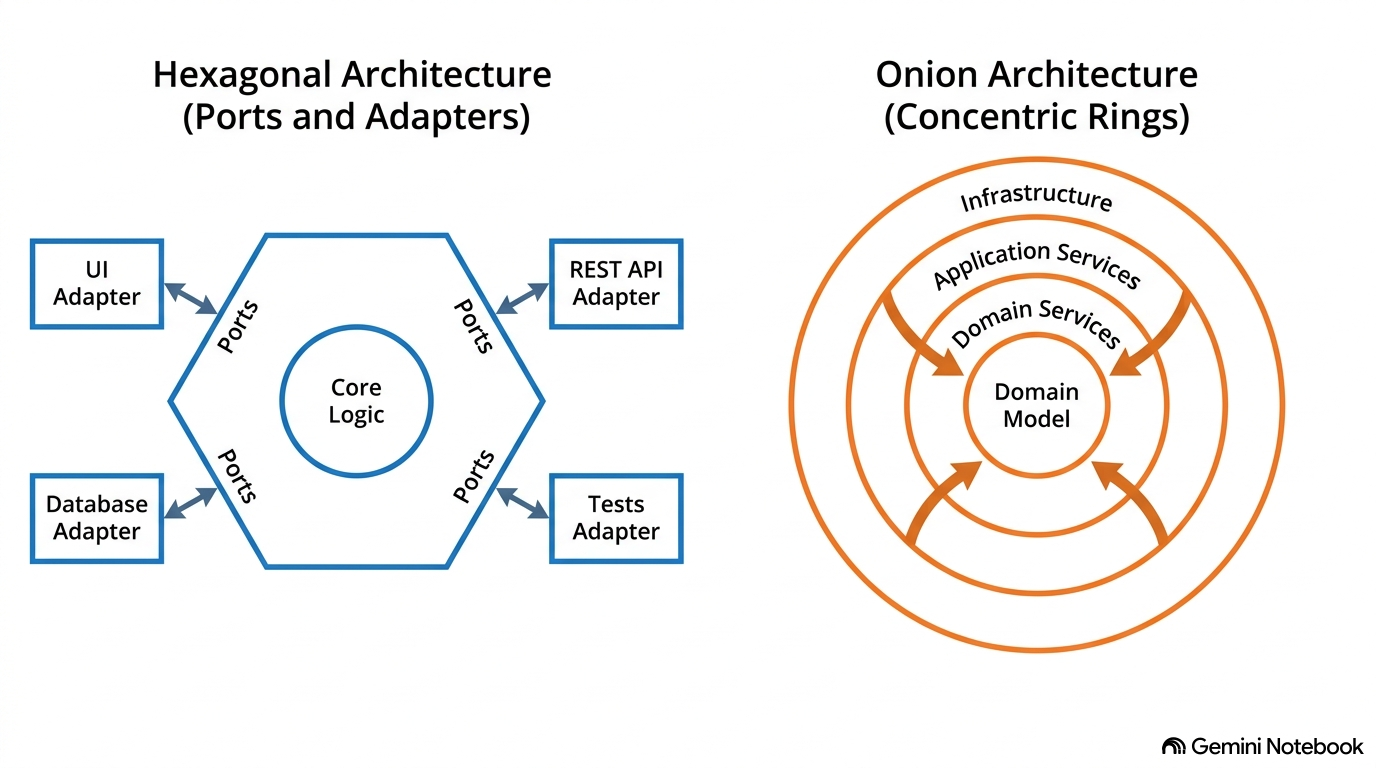
\includegraphics[width=\linewidth]{hexagonal_vs_onion.png}
    \caption{Comparación visual entre la simetría del hexágono y la jerarquía de capas de Onion.}
    \label{fig:hexagonal-vs-onion}
\end{figure}

\subsubsection*{2. Geometría del hexágono: eliminación de ejes de asimetría}

Cockburn enfatiza que la elección de una figura geométrica de seis lados \textbf{no responde a una razón numérica} (el sistema no está limitado a seis componentes, seis puertos o seis tecnologías) \parencite{cockburn2005hexagonal}. El propósito de utilizar un hexágono es \textbf{romper deliberadamente con la metáfora unidimensional} propia de las capas apiladas («arriba-abajo») o de los diagramas de tuberías («izquierda-derecha») \parencite{cockburn2005hexagonal}. Un esquema rectangular tienta visualmente a encasillar «entradas por la izquierda» y «salidas por la derecha». El hexágono proporciona múltiples aristas simétricas e independientes para dibujar y distribuir puertos y adaptadores (UI, DB, servicios REST, tests, mensajes) en diversas direcciones alrededor del núcleo, evidenciando que el dominio no depende de ningún medio de transporte o almacenamiento en particular \parencite{cockburn2005hexagonal,martin2017clean}.

\subsubsection*{3. Traducción de «Puerto y Adaptador» en las capas internas de Onion}

En la Arquitectura Onion de Palermo, el sistema se estructura en capas o anillos concéntricos alrededor del \emph{Domain Model} y los \emph{Domain Services}, los cuales son rodeados por los \emph{Application Services} y la capa externa de \emph{Infrastructure} \parencite{palermo2008onion}. El concepto de \textbf{Puerto y Adaptador} se traduce operacionalmente en la Arquitectura Onion mediante la aplicación estricta del \textbf{Principio de Inversión de Dependencias (DIP)} y la \textbf{Regla de Dependencia} \parencite{palermo2008onion,martin2017clean}:

\begin{itemize}
    \item \textbf{Puerto $\equiv$ Interfaz abstracta en capas internas (Core):} En Onion, un \emph{Puerto} es un contrato de interfaz definido en las capas del centro (dentro del \emph{Domain} o \emph{Application Services}) \parencite{palermo2008onion,cockburn2005hexagonal}. Por ejemplo, la interfaz \texttt{IOrderRepository} o \texttt{IPaymentGateway} se declara dentro del núcleo y especifica \emph{qué} requiere el dominio sin depender de detalles de implementación \parencite{palermo2008onion}.
    \item \textbf{Adaptador $\equiv$ Clase concreta en la capa externa (Infrastructure):} Un \emph{Adaptador} es la implementación concreta de dicha interfaz, la cual reside exclusivamente en el anillo periférico de \emph{Infrastructure} o \emph{UI} \parencite{palermo2008onion,cockburn2005hexagonal}. Por ejemplo, \texttt{SqlOrderRepository} (que implementa \texttt{IOrderRepository}) o \texttt{StripeAdapter}.
\end{itemize}

Dado que en Onion todas las dependencias del código fuente apuntan obligatoriamente hacia el centro \parencite{palermo2008onion}, la infraestructura externa depende de la interfaz definida en el núcleo interno. Así, se garantiza la total independencia y testabilidad del dominio frente a cambios tecnológicos \parencite{palermo2008onion,martin2017clean}.
